\documentclass[40pt, a0paper, portrait, margin=0mm, innermargin=10mm,
blockverticalspace=-2mm]{tikzposter}

\geometry{}
\usepackage{amsmath}
\usepackage{enumerate}

\definecolor{royalblue}{RGB}{19,42,80}
\definecolor{skyblue}{RGB}{70,150,150}
\definecolor{mygreen}{RGB}{50,185,85}

\definecolorstyle{myColorStyle} {
    \colorlet{colorOne}{royalblue}
    \colorlet{colorTwo}{skyblue}
    \colorlet{colorThree}{white}
    }{
    % Background Colors
    \colorlet{backgroundcolor}{colorTwo!45}
    % \colorlet{backgroundcolor}{mygreen}
    \colorlet{framecolor}{colorTwo!30}
    % Title Colors
    \colorlet{titlefgcolor}{white}
    \colorlet{titlebgcolor}{colorOne}
    % Block Colors
    \colorlet{blocktitlebgcolor}{colorTwo!45}
    \colorlet{blocktitlefgcolor}{black}
    \colorlet{blockbodybgcolor}{colorTwo!45}
    \colorlet{blockbodyfgcolor}{black}
    % Innerblock Colors
    \colorlet{innerblocktitlebgcolor}{white}
    \colorlet{innerblocktitlefgcolor}{black}
    \colorlet{innerblockbodybgcolor}{white}
    \colorlet{innerblockbodyfgcolor}{black}
    % Note colors
    \colorlet{notefgcolor}{black}
    \colorlet{notebgcolor}{white}
    \colorlet{notefrcolor}{white}
}

\usecolorstyle{myColorStyle}
\usetitlestyle{Empty}
\useblockstyle{Minimal}


% \usepackage{avant}
\renewcommand*\familydefault{lmr}
% \usepackage[utf8]{fontenc}
\usepackage{fix-cm}
\usepackage{tikz}
\usepackage{multicol}


\makeatletter
\newcommand\semiHUGE{\@setfontsize\semiHUGE{96}{27.38}}
\newcommand\semiHuge{\@setfontsize\semiHuge{48}{27.38}}
\makeatother

\DeclareSymbolFont{extraup}{U}{zavm}{m}{n}
\DeclareMathSymbol{\vardiamond}{\mathalpha}{extraup}{87}


\title{\parbox{\linewidth}{\centering \textnormal{\semiHUGE Predicting phytoplankton growth
from metabolic rates}}}
\author{\semiHuge \textbf{Bernardo Garc{\'i}a-Carreras$^*$, Gabriel Yvon-Durocher$^\dagger$} 
\textit{\&} \textbf{Samraat Pawar$^*$}\\
\vspace{0.5cm}
{\LARGE \texttt{bgarciacarreras@gmail.com}}}
\institute{$^*$Imperial College London, Silwood Park, UK \hspace{1cm} |
    \hspace{1cm} $^\dagger$University of Exeter, Penryn, UK}


\sloppy

\clubpenalty=9999
\widowpenalty=9999



\begin{document}

\node[xshift=-42.05cm, at=(topright),opacity=0.9] {
\includegraphics[width=\paperwidth]{../figs/head.jpg}}


\maketitle[titletoblockverticalspace=0mm]

\vspace{-2cm}

\begin{columns}
\column{0.5}
\block[bodyverticalshift=-14mm]{\textbf{I.} \textit{Introduction}}{
    \coloredbox{\LARGE
        \centering
        \vspace{0.4cm}
        \begin{minipage}[]{0.95\linewidth}
            \vspace{0.25cm}
            \begin{minipage}[]{0.65\linewidth}
                Exponential growth is a measure of fitness in competition and
                evolution. Growth is partly determined by \textit{net flux}
                (balance between $P_\text{gross}$ and $R$ determining the
                available carbon). $P_\text{gross}$ and $R$ respond to
                temperature.
            \end{minipage} \hspace{0.25cm} \begin{minipage}[]{0.32\linewidth}
                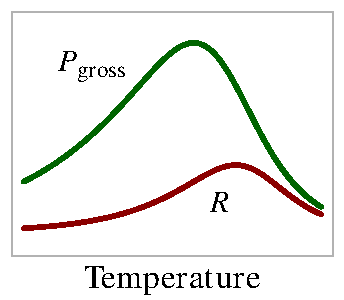
\includegraphics[width=\linewidth]{figs/gp_r_av.pdf}
            \end{minipage} 
            \vspace{0.6cm}

            Additional temperature dependent factors may mediate how the
            available carbon is translated into growth, such as efficiency,
            allocations to growth, or nutrient uptake.
            \vspace{1cm}

            We ask two broad questions:
            \vspace{0.4cm}
            \begin{enumerate}[(i)]
                \item \textit{\bfseries{How might $P_\textnormal{gross}$ and $R$
                    combine to determine the temperature response of growth?}} 
                \item \textit{\bfseries{How could other mediating factors
                    further affect growth's response to temperature?}} \\
            \end{enumerate}
            \vspace{-0.6cm}
        \end{minipage}
    }
}


\block[bodyverticalshift=-14mm]{\textbf{III.} {\textit{Results: mismatch in
    metabolic rates}}}{
    \coloredbox{
        \begin{minipage}[]{0.43\linewidth}
            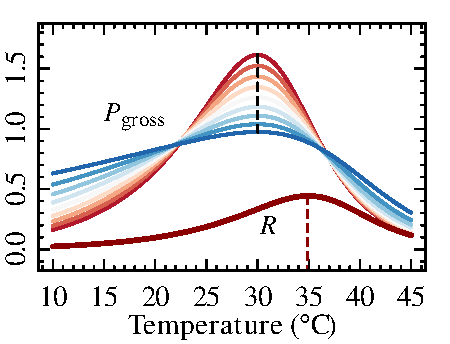
\includegraphics[width=\linewidth]{figs/gp_r_gen_spe_art.pdf}
        \end{minipage} \hspace{0.25cm} \begin{minipage}[]{0.52\linewidth}
            \LARGE $P_\text{gross}$ changes from a specialist (red) profile
            sharing the same activation energy as $R$, to a generalist (blue)
            curve.
        \end{minipage}

        \vspace{1cm}
        \begin{minipage}[]{\linewidth}
            \begin{center}
                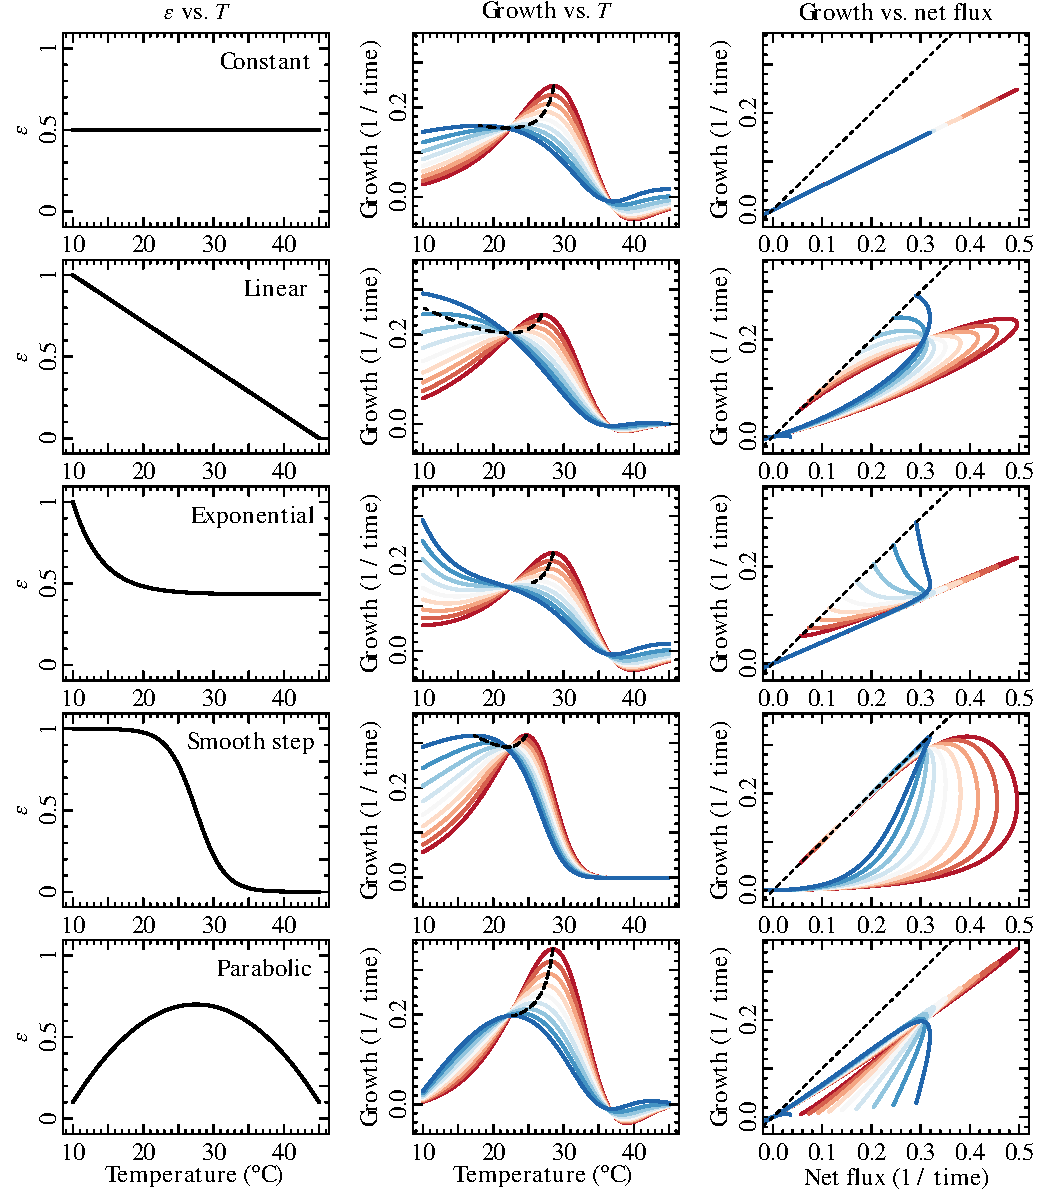
\includegraphics[width=\linewidth]{figs/loopy_business_gen_spe.pdf}
            \end{center}
        \end{minipage}
        \vspace{0.8}
    }
}



\block[bodyverticalshift=-4mm]{}{
    \coloredbox{
        \centering
        \begin{minipage}{0.98\linewidth}
            \large
            \vspace{0.2cm}
            \begin{itemize}
                \item Padfield \textit{et al.} (2016). Rapid evolution of
                    metabolic traits explains thermal adaptation in
                    phytoplankton. \textit{Ecol. Lett.} 19:133--142.
                \item Kempes \textit{et al.} (2012). Growth, metabolic
                    partitioning, and the size of microorganisms. \textit{PNAS}
                    109:495--500.
            \end{itemize}
            \vspace{0.3cm}
        \end{minipage}
    }
}


\column{0.5}

\block[bodyverticalshift=-17mm]{\textbf{II.} \textit{Model \& approach}}{
    \coloredbox{\LARGE
        \centering
        \vspace{0.4cm}
        \begin{minipage}[]{0.95\linewidth}
            Over the course of a 24 hour period, exponential growth $r$ is 
            \begin{equation*}
                r = \varepsilon \, (P_\text{gross} - R_\text{light} -
                R_\text{dark}),
            \end{equation*}
            % \vspace{0.22cm}
            where $\varepsilon$ is, potentially, any combination of (possibly)
            temperature dependent factors mediating how carbon is translated to
            growth. We idealise $\varepsilon$ with five generic functions:
            \vspace{-1.5cm}

            \begin{center}
                constant {\normalsize $\vardiamond$} 
                linear {\normalsize $\vardiamond$} 
                exponential {\normalsize $\vardiamond$} 
                smooth step {\normalsize $\vardiamond$} parabolic
            \end{center}
            \vspace{0.5cm}
        \end{minipage}
    }
}


\block[bodyverticalshift=-14mm]{\textbf{IV.} {\textit{Results: $\varepsilon$'s contribution}}}{
    \coloredbox{\LARGE
        \centering
        \vspace{0.4cm}
        \begin{minipage}[]{0.95\linewidth}
            By using the intermediate curve of $P_\text{gross}$ from
            \textbf{III.}, and instead varying the intensity of $\varepsilon$,
            we can show $\varepsilon$'s contribution to shifts in the growth
            curve.
        \end{minipage}

        \vspace{0.85cm}

        \begin{minipage}[]{\linewidth}
        \begin{center}
            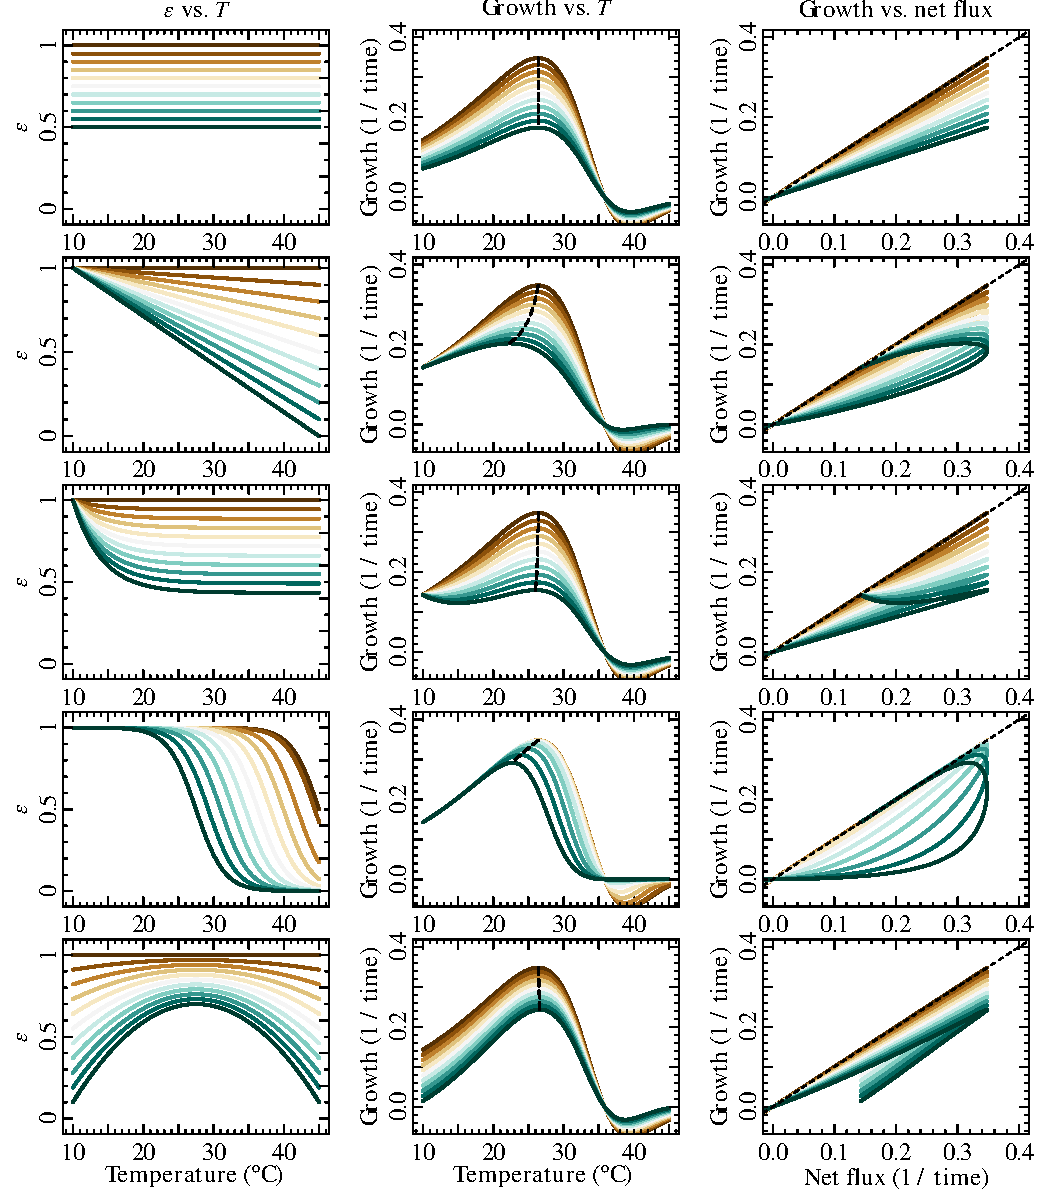
\includegraphics[width=\linewidth]{figs/loopy_business_gen_spe_eps.pdf}
        \end{center}
        \end{minipage}
        \vspace{0.1cm}
    }
}


\block[bodyverticalshift=-14mm]{{\textbf{V.} \textit{Summary}}}{
    \coloredbox{\LARGE
        \centering
        \vspace{0.4cm}
        \begin{minipage}[]{0.42\textwidth}
            \begin{itemize}
                \item As the differences between the shapes of the
                    $P_\text{gross}$ and $R$ curves becomes more pronounced, the
                    temperature response of growth is increasingly affected.
                \item Adding a temperature dependent factor $\varepsilon$ can
                    exacerbate impacts on the growth curve.
                \item Preliminary experimental data suggests $\varepsilon$ is
                    temperature dependent, and either linear or exponential.
            \end{itemize}
        \end{minipage}
        \vspace{0.2cm}
    }
}


\block[bodyverticalshift=-14mm]{{\textbf{VI.} \textit{Ongoing work}}}{
    \coloredbox{\LARGE
        \centering
        \vspace{0.4cm}
        \begin{minipage}[]{0.43\textwidth}
            \begin{itemize}
                \item Experimental parameterisation and validation is underway.
                \item How do assumptions made about $\varepsilon$ affect
                    predictions of fitness differentials between two competing
                    species based on metabolic rates alone?
            \end{itemize}
        \end{minipage}
        \vspace{0.2cm}
    }
}

\end{columns}

\end{document}

